%%%%%%%%%%%%%%%%%%%%%%%%%%%%% Define Article %%%%%%%%%%%%%%%%%%%%%%%%%%%%%%%%%%
\documentclass{article}
%%%%%%%%%%%%%%%%%%%%%%%%%%%%%%%%%%%%%%%%%%%%%%%%%%%%%%%%%%%%%%%%%%%%%%%%%%%%%%%

%%%%%%%%%%%%%%%%%%%%%%%%%%%%% Using Packages %%%%%%%%%%%%%%%%%%%%%%%%%%%%%%%%%%
\usepackage{geometry}
\usepackage{graphicx}
\usepackage{amssymb}
\usepackage{amsmath}
\usepackage{amsthm}
\usepackage{empheq}
\usepackage{mdframed}
\usepackage{booktabs}
\usepackage{lipsum}
\usepackage{graphicx}
\usepackage{color}
\usepackage{psfrag}
\usepackage{pgfplots}
\usepackage{bm}
%%%%%%%%%%%%%%%%%%%%%%%%%%%%%%%%%%%%%%%%%%%%%%%%%%%%%%%%%%%%%%%%%%%%%%%%%%%%%%%

% Other Settings

%%%%%%%%%%%%%%%%%%%%%%%%%% Page Setting %%%%%%%%%%%%%%%%%%%%%%%%%%%%%%%%%%%%%%%
\geometry{a4paper}

%%%%%%%%%%%%%%%%%%%%%%%%%% Define some useful colors %%%%%%%%%%%%%%%%%%%%%%%%%%
\definecolor{ocre}{RGB}{243,102,25}
\definecolor{mygray}{RGB}{243,243,244}
\definecolor{deepGreen}{RGB}{26,111,0}
\definecolor{shallowGreen}{RGB}{235,255,255}
\definecolor{deepBlue}{RGB}{61,124,222}
\definecolor{shallowBlue}{RGB}{235,249,255}
%%%%%%%%%%%%%%%%%%%%%%%%%%%%%%%%%%%%%%%%%%%%%%%%%%%%%%%%%%%%%%%%%%%%%%%%%%%%%%%

%%%%%%%%%%%%%%%%%%%%%%%%%% Define an orangebox command %%%%%%%%%%%%%%%%%%%%%%%%
\newcommand\orangebox[1]{\fcolorbox{ocre}{mygray}{\hspace{1em}#1\hspace{1em}}}
%%%%%%%%%%%%%%%%%%%%%%%%%%%%%%%%%%%%%%%%%%%%%%%%%%%%%%%%%%%%%%%%%%%%%%%%%%%%%%%

%%%%%%%%%%%%%%%%%%%%%%%%%%%% English Environments %%%%%%%%%%%%%%%%%%%%%%%%%%%%%
\newtheoremstyle{mytheoremstyle}{3pt}{3pt}{\normalfont}{0cm}{\rmfamily\bfseries}{}{1em}{{\color{black}\thmname{#1}~\thmnumber{#2}}\thmnote{\,--\,#3}}
\newtheoremstyle{myproblemstyle}{3pt}{3pt}{\normalfont}{0cm}{\rmfamily\bfseries}{}{1em}{{\color{black}\thmname{#1}~\thmnumber{#2}}\thmnote{\,--\,#3}}
\theoremstyle{mytheoremstyle}
\newmdtheoremenv[linewidth=1pt,backgroundcolor=shallowGreen,linecolor=deepGreen,leftmargin=0pt,innerleftmargin=20pt,innerrightmargin=20pt,]{theorem}{Theorem}[section]
\theoremstyle{mytheoremstyle}
\newmdtheoremenv[linewidth=1pt,backgroundcolor=shallowBlue,linecolor=deepBlue,leftmargin=0pt,innerleftmargin=20pt,innerrightmargin=20pt,]{definition}{Definition}[section]
\theoremstyle{myproblemstyle}
\newmdtheoremenv[linecolor=black,leftmargin=0pt,innerleftmargin=10pt,innerrightmargin=10pt,]{problem}{Problem}[section]
%%%%%%%%%%%%%%%%%%%%%%%%%%%%%%%%%%%%%%%%%%%%%%%%%%%%%%%%%%%%%%%%%%%%%%%%%%%%%%%

%%%%%%%%%%%%%%%%%%%%%%%%%%%%%%% Plotting Settings %%%%%%%%%%%%%%%%%%%%%%%%%%%%%
\usepgfplotslibrary{colorbrewer}
\pgfplotsset{width=8cm,compat=1.9}
%%%%%%%%%%%%%%%%%%%%%%%%%%%%%%%%%%%%%%%%%%%%%%%%%%%%%%%%%%%%%%%%%%%%%%%%%%%%%%%

%%%%%%%%%%%%%%%%%%%%%%%%%%%%%%% Title & Author %%%%%%%%%%%%%%%%%%%%%%%%%%%%%%%%
\title{Parcial 1 - METODOS NÚMERICOS}
\author{Rodrigo Alexander Miranda Ramirez MR181415}
%%%%%%%%%%%%%%%%%%%%%%%%%%%%%%%%%%%%%%%%%%%%%%%%%%%%%%%%%%%%%%%%%%%%%%%%%%%%%%%

\begin{document}
    \maketitle
%%%%%%%%%%%%%%%%%%%%%%%%%%%%%EJERCICIO 1%%%%%%%%%%%%%%%%%%%%%%%%%%%%%%%%%%%%%%%%%
    \begin{figure}[ht]
        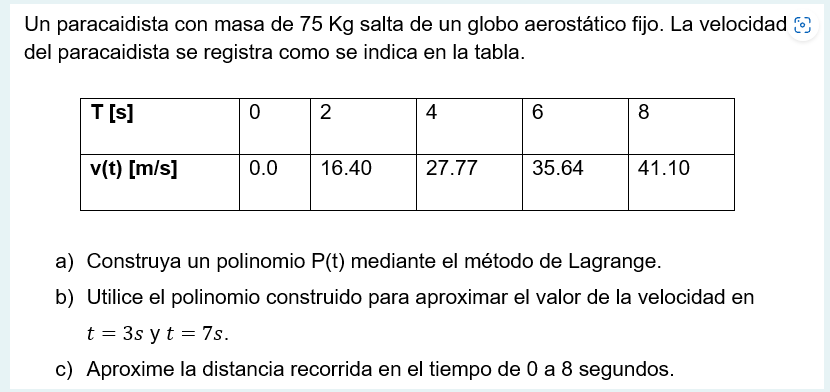
\includegraphics[scale=0.8]{img/eje1_1.png}
     \end{figure}


\pagebreak
\noindent \\ 
\\ Velocidad en $t=3s$
\begin{figure}[ht]
    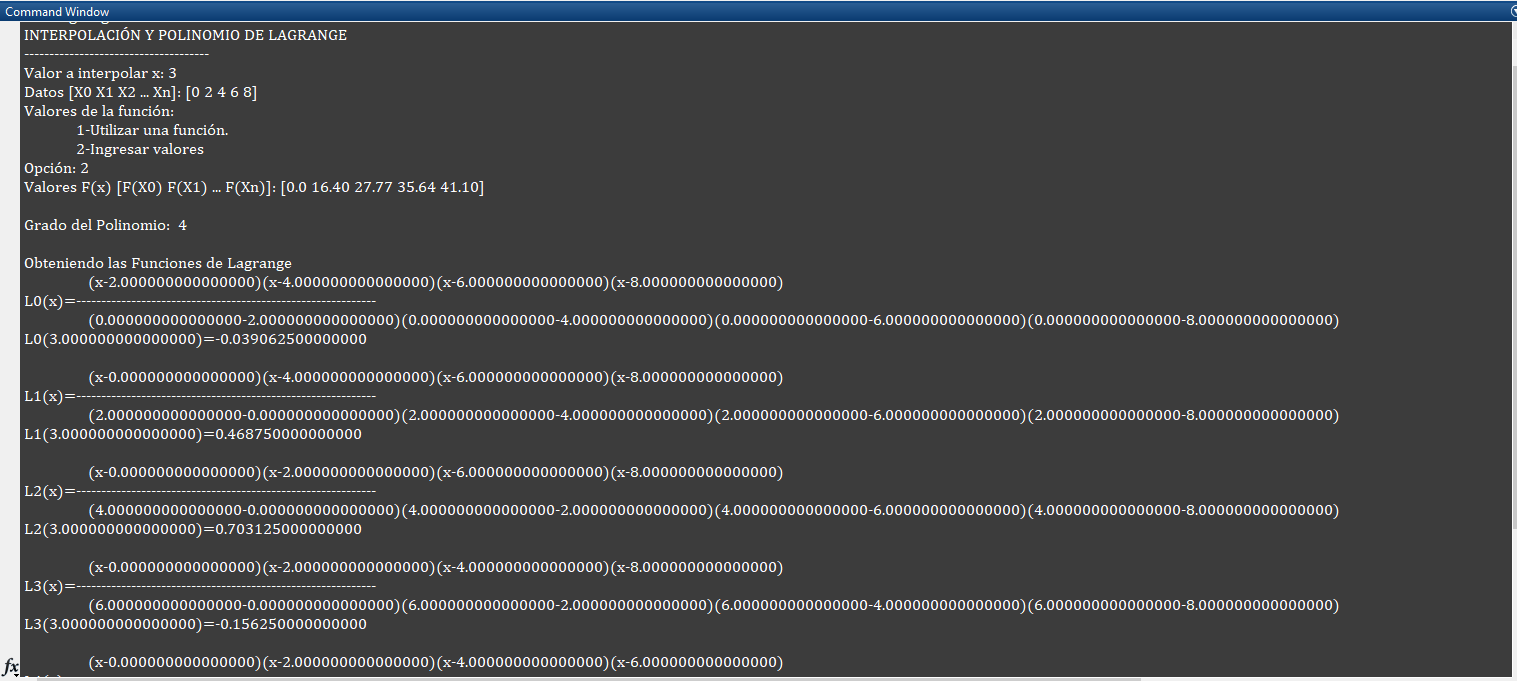
\includegraphics[scale=0.6]{img/eje1_3.png} \\
    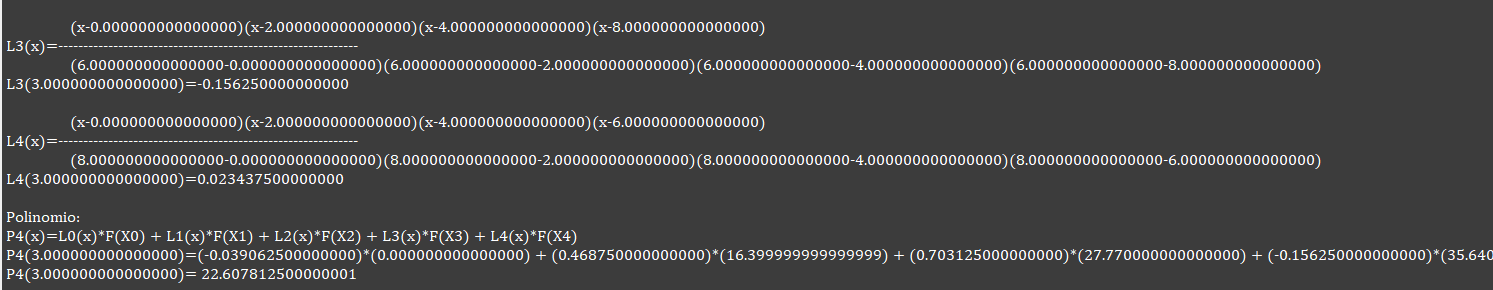
\includegraphics[scale=0.6]{img/eje1_4.png}
\end{figure}
\\La velocidad en $t=3s$ es de $22.607812500000001$
\pagebreak
\noindent \\Velocidad en $t=7s$
\begin{figure}[ht]
    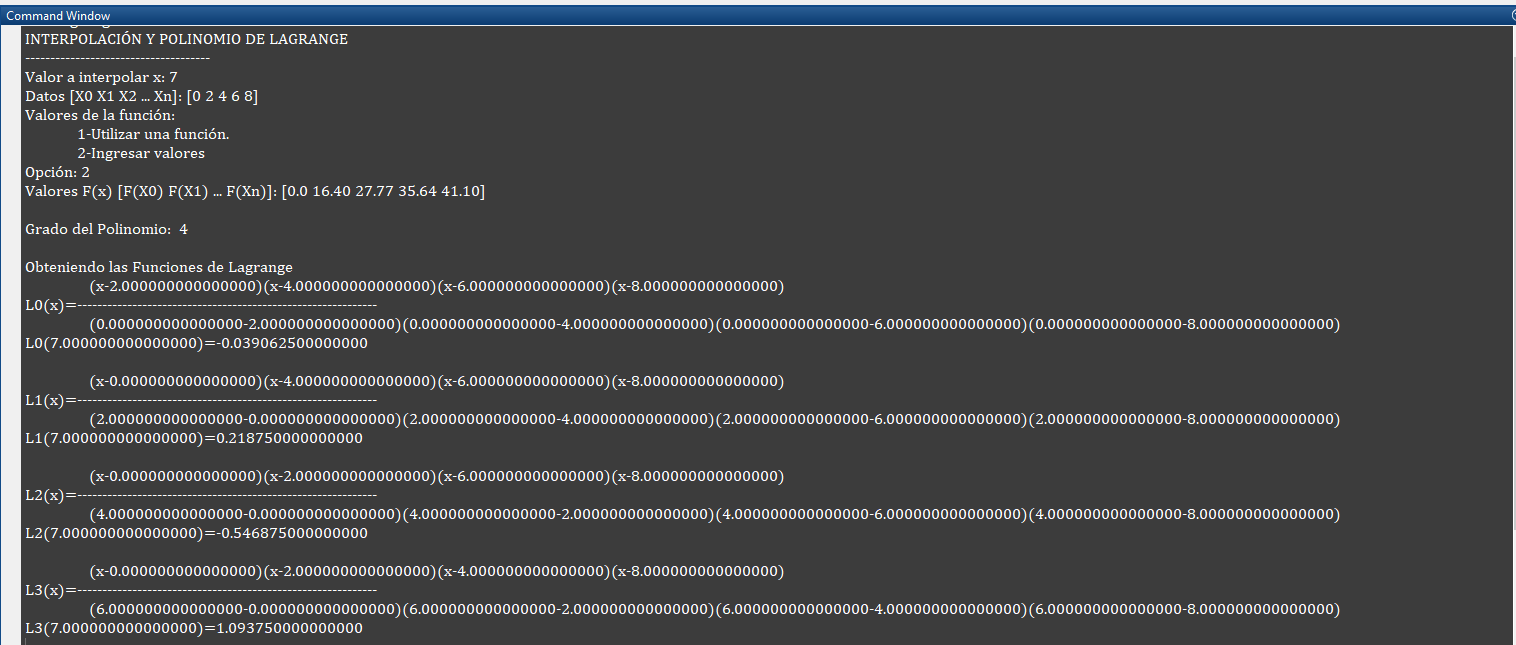
\includegraphics[scale=0.6]{img/eje1_5.png} \\
    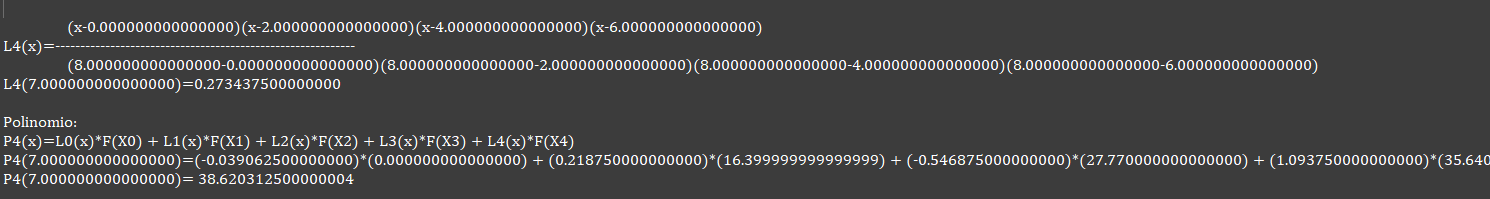
\includegraphics[scale=0.6]{img/eje1_6.png}
\end{figure}
\\La velocidad en $t=7s$ es de $38.620312500000004$
\noindent \\ La distancia recorrida en el tiempo de 0 a 8 segundos 
\\$x=x0+v*t= 0+41.10*8=328.8m$
%%%%%%%%%%%%%%%%%%%%%%EJERCICIO 2%%%%%%%%%%%%%%%%%%%%%%%%%%%%%%%%%%%%%%%%%%%%%%%%%%%
\pagebreak
\begin{figure}[ht]
    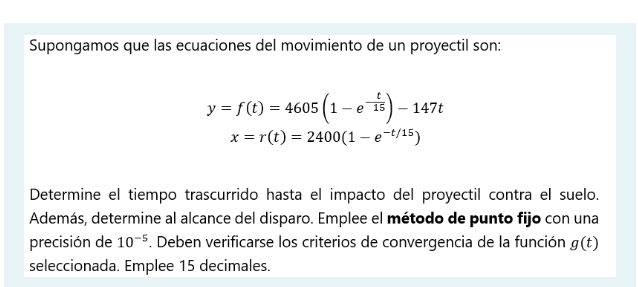
\includegraphics[scale=0.8]{img/eje2_1.png}
 \end{figure}
\noindent \\Cuando impacta contra el suelo h=0 v=0
\\Declarando las ecuaciones en matlab:
\begin{figure}[ht]
    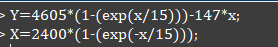
\includegraphics[scale=0.7]{img/eje2_2.png}
 \end{figure}
\\Determinando el tiempo transcurrido hasta el impacto en el suelo
\begin{figure}[ht]
    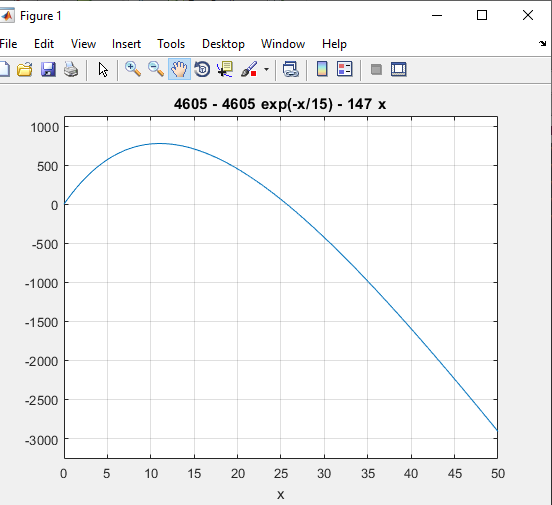
\includegraphics[scale=0.6]{img/eje2_3.png}
\end{figure}
\\Escribiremos la funcion de la forma $t=4605(1-e^(-t/15))/14$ 
\\Observamos que el intervalo donde golpea el suelo es[25 26]. Vamos matlab
 \begin{figure}[ht]
    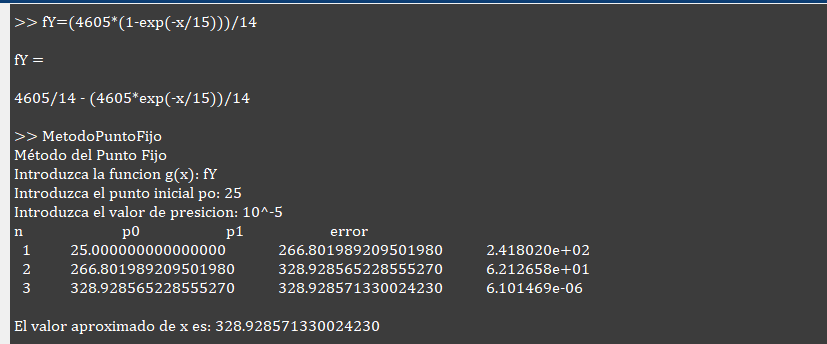
\includegraphics[scale=0.6]{img/eje2_4.png}
\end{figure}
\\Impactara el suelo en $t=328.92$
\\El Alcance es de: $3.289285713300242e+02$
\begin{figure}[ht]
    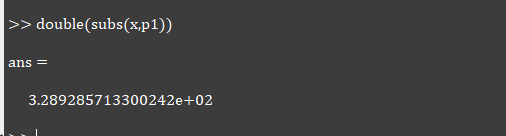
\includegraphics[scale=0.6]{img/eje2_5.png}
\end{figure}

%%%%%%%%%%%%%%%%%%%%%%%%%EJERCICIO 3%%%%%%%%%%%%%%%%%%%%%%%%%%%%%%%%%%%%%%%%
\pagebreak
\begin{figure}[ht]
    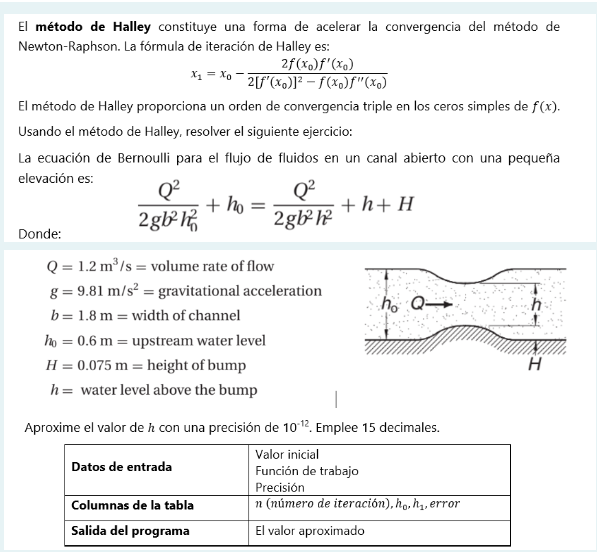
\includegraphics[scale=0.8]{img/eje3_1.png} \\
    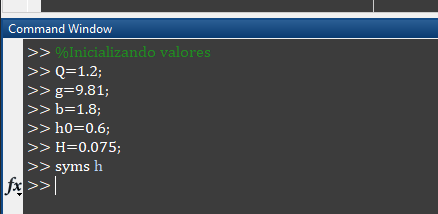
\includegraphics[scale=0.7]{img/eje3_2.png}
\end{figure}
\noindent \\ Una vez declaradas la variables en Matlab, y modificado el codigo, lo ejecutaremos para obtener la respuesta
\\Declaramos fun:
\begin{figure}[ht]
    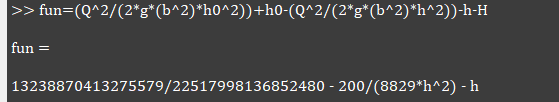
\includegraphics[scale=0.7]{img/eje3_3.png}{\\Graficamos para determinar el punto a evaluar:}
\end{figure}

\begin{figure}[ht]
    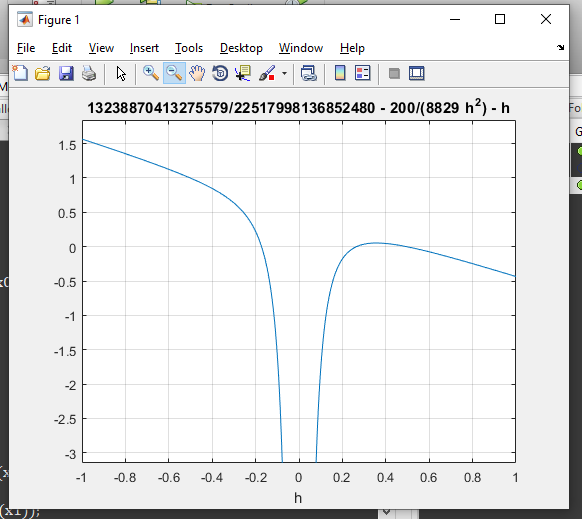
\includegraphics[scale=0.6]{img/eje3_4.png}{\\El punto que usaremos sera 0.2}
\end{figure}

\begin{figure}[ht]
    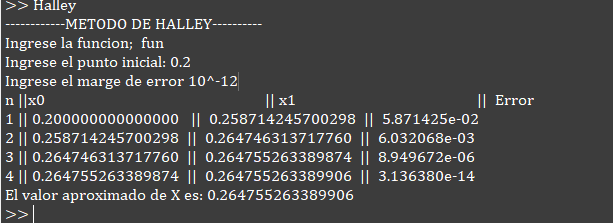
\includegraphics[scale=0.7]{img/eje3_5.png}{\\$h=0.264755263389906$}
\end{figure}


%%%%%%%%%%%%%%%%%%EJERCICIO 4%%%%%%%%%%%%%%%%%%
\pagebreak
\begin{figure}[ht]
    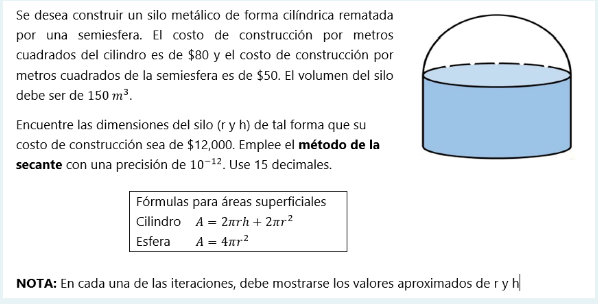
\includegraphics[scale=0.8]{img/eje4_1.png} 
\end{figure}








\end{document}
